\documentclass[a4paper]{article}
\usepackage[a4paper,  margin=1.0in]{geometry}

\usepackage{graphicx}
\usepackage{float}
\usepackage{hyperref}
\usepackage{listings}
\lstset{
basicstyle=\small\ttfamily,
columns=flexible,
breaklines=true
}

\usepackage{polski}
\usepackage[utf8]{inputenc}
\begin{document}


\title{Ćwiczenie nr 2 z MBI, adnotacja DNA}
\author{Jakub Skałecki, Kinga Kimnes}
\maketitle

\section{Przygotowanie danych}
W ramach doświadczenia wykorzystano, uzyskany wskutek assemblingu, genom tasiemca (hymenolepis diminuta), zawierający całościowo 3035 kontigów (scaffoldów). W przeprowadzonym badaniu wykorzystany został kontig fizyczny o identyfikatorze:
\begin{verbatim}
> HDID_scaffold0000073 length=149394,
\end{verbatim}
spełniający warunek odznaczania się długością powyżej 100kbp (149394kbp).

\section{Maskowanie genomu}

W dalszej kolejności przeprowadzono maskowanie genomu, polegające na wygenerowaniu zmodyfikowanej sekwencji DNA, zawierającej zamaskowane powatrzające się sekwencje.
W tym celu wykorzystano program RepeatMasker, sprawdzający fragmenty DNA pod kątem powtórzeń, jak i sekwencji o niskiej złożoności. Dane wyjściowe stanowią: szczegółowa adnotacja powtórzeń obecnych w sekwencji zapytań wraz ze zemodyfikowaną wersją sekwencji, w której zamaskowano wszelkie powtórzenia (wstawiając w miejscach tych literę N). Działanie programu oparte jest o algorytm Smitha-Watermana-Gotoh'a
Liczba uzyskanych, zamaskowanych nukleotydów wyniosła w naszej próbie 2296.

\section{Mapowanie znanych sekwencji i adnotacja strukturalna}

W kolejnym etapie dokonano adnotacji strukturalnej, dostarczającej danych usprawniających identyfikację struktur genowych. Dzięki zastosowaniu programu Make, w efekcie przyrównania białek i mRNA do genomu (ich zmapowania), uzyskano adnotacje genów w formacie GFF3.
Poniżej zamieszczono 10 pierwszych linii, wygenerowanego przez program Maker, pliku gff:
\begin{lstlisting}
##gff-version 3
HDID_scaffold0000073	.	contig	1	149394	.	.	.	ID=HDID_scaffold0000073;Name=HDID_scaffold0000073
###
HDID_scaffold0000073	repeatmasker	match	32910	32976	263	+	.	ID=HDID_scaffold0000073:hit:0:1.3.0.0;Name=species:NONAUT-5|genus:LTR%2FGypsy;Target=species:NONAUT-5|genus:LTR%2FGypsy 1346 1412 +
HDID_scaffold0000073	repeatmasker	match_part	32910	32976	263	+	.	ID=HDID_scaffold0000073:hsp:0:1.3.0.0;Parent=HDID_scaffold0000073:hit:0:1.3.0.0;Target=species:NONAUT-5|genus:LTR%252FGypsy 1346 1412 +
HDID_scaffold0000073	repeatmasker	match	33324	33816	718	+	.	ID=HDID_scaffold0000073:hit:1:1.3.0.0;Name=species:NONAUT-3|genus:LTR%2FGypsy;Target=species:NONAUT-3|genus:LTR%2FGypsy 1606 2102 +
HDID_scaffold0000073	repeatmasker	match_part	33324	33816	718	+	.	ID=HDID_scaffold0000073:hsp:1:1.3.0.0;Parent=HDID_scaffold0000073:hit:1:1.3.0.0;Target=species:NONAUT-3|genus:LTR%252FGypsy 1606 2102 +
HDID_scaffold0000073	repeatmasker	match	33918	34592	492	+	.	ID=HDID_scaffold0000073:hit:2:1.3.0.0;Name=species:Gypsy2_MH-I|genus:LTR%2FGypsy;Target=species:Gypsy2_MH-I|genus:LTR%2FGypsy 2392 3335 +
HDID_scaffold0000073	repeatmasker	match_part	33918	34592	492	+	.	ID=HDID_scaffold0000073:hsp:2:1.3.0.0;Parent=HDID_scaffold0000073:hit:2:1.3.0.0;Target=species:Gypsy2_MH-I|genus:LTR%252FGypsy 2392 3335 +
HDID_scaffold0000073	repeatmasker	match	34932	35128	262	+	.	ID=HDID_scaffold0000073:hit:3:1.3.0.0;Name=species:GYPSY1-I_CB|genus:LTR%2FGypsy;Target=species:GYPSY1-I_CB|genus:LTR%2FGypsy 3101 3300 +
\end{lstlisting}

Przykładowa adnotacja typu \texttt{expressed\_sequence\_match} w pliku .gff (wygenerowanym przez program Maker):
\begin{lstlisting}
HDID_scaffold0000073	blastn	expressed_sequence_match	1868	12755	887	+	.	ID=HDID_scaffold0000073:hit:11:3.2.0.0;Name=HDID_0000755601-mRNA-1
\end{lstlisting}

Jej źródłemi jest program blastn, służący do porównywania sekwencji z bazą danych sekwencji nukleotydowych.
W naszym przypadku bazą danych jest plik z sekwencją mRNA dla tasiemca
(sekwencja dopasowana została do scaffoldu o identyfikatorze \texttt{HDID\_0000755601-mRNA-1}).


Nukleotydy tej sekwencji:

\begin{verbatim}
ATGGCTCAAGAAGATGATGATCGTAATCTTCTTATGATCTTAATTGATCTTACCCCAGTG
TGGTGGGGTACTTATGCTCACGAGTTTCTTATTCTTCCCACATTCATCGAAAATATTCTC
GCTTTCGCCAATAGTCATTTGGCTCTATCACCCCTTAATGAGGTAGCAATTGTTGGCGTA
ACTCCCGAGAAAACCGAATTTTTATGGCCTTCTCTAAACCCCATTGATGAAATTGAATGC
CACAATGGTCAGTATGAACCGTTCTCGATTATCGGTCAAACAGTACGAAAGAAAGTCAAC
CAGATGATTATGTCCTGTGAGTCGACGAGATGTACGGTCGCTTTCGCTAATGCGATTAAT
AACGCTCTTTGTTACTTCATTCGTCGCTGTCGAGAAATGCGTCCTACTTTTGCTTACACT
CGAATCGATTCAAATACATTGATGGAGGATGACATTCATAGTCTGCTGAAGGACAATTTC
CATGCTCGGATTCTTGTCGTTCGAGCGGCTGAGGATGATTCTTCTCAATACCTTTCTCTC
ATGAATGCTGTCTTTACCGCTCAAAAGATGGGAGTGCTGATCGACGCTTGTATTATACCC
CCTACTCGAATGTCTTACTCCACCGAAGATCATCTTCGTCAATCATCCACAACTCTCCAG
GAGTCTGGACATTCTAGTCTCTTCCAACAAGCTGCGGAACTGACTGGAGGTATTTATCTT
CGTATTCCGAGACCTGCAGGACTTTTACAGTACCTCCTTTGTGTTTTTCTCCCGCATGCA
GGTCTCAGATCTCAAATGATCCTTCCAGATTCTAATGGGGGCTCATCTGCAGGGGTGGAT
TTTCGTTCGGCCTGTTTTTGTCACCACAAGATGGTCGATTTAGCTTATGTTTGCTCTGTC
TGCCTGTCTGTATTCTGTGAATTCTCTCCTATCTGTTCAACTTGTCAAACTCCTTTTCGC
ATTCCCACTTCTGTAACTCTACCTCCTGAGAAGCTCAAAAATGTAAAATAAATATCTTCT
GTTTCTCAATTGCTCTTCGGCTTTTTTGATATTCCGTTTGGTTACTTTTGTTCTAATCTT
ACCTTGGTTGTTTCAGCGCGAAGATGGATTCAGATGATATCTTGCCATCAAAACGCATTA
AGGTATTAAAATAGTTCTTTTCTTTAAGATGAAGAACGTGATTTAAGTCTTGTTGAATAA
TTAGTTTATTTCTTCACTCCTTCCACATTTGTAGGTTGATGATACCCAAATCGGTTCCAA
GGGTTGGGACTTGATGGTGAGTTATCGCTTAATAAGTGGATTTGGAACTTTGTTCCTAAT
TATTTTGCTCTGTTGTGGACGGGAGCTGTCGATTTTCTCCTCGTCTGGGGATTTTGATTT
TGATTAATGCTGAGCCCTAAGCACAGATTAGTTAGTTAGTCTGTTAGTCTGTTAATGTAA
GGTAAAATCATCTAAGCTCAACTAATATGTCAAAAACTGAGGAGATGTGGTATCCAAGGC
TGCAAATTCAAATTTTGCTTTCAAGTTCATTGGTGAAAATCGTCTTCCAAGATGTTTATA
TTCGAGGATAAAAGCACTTCCATTTTTTCTAACTAGTTCATTTGCGCTAAACGAAAATCA
TAGCTCAATGCCTATGATTTCTCTGCTACTATGGGAGTAAGACGGGGGCCACCACTCAAG
ATTTCTTTTGCTAAAAATGAATTAGAGCTGGATTGTTAAATATGCTGCAATATACAATTA
GCGCTTCCCATTGCTAAATGAAATGTCCACTGTATTAAACTGCTAAAGTCTGGGATATCT
AGAATTATCATCCCGTAGCTGCTAAATTGCTTTTCCCAGTGCATTTTAATTTAAAAGACG
AGAAAGTAACTGTAACGTCTATTAGATACACTGCGTAAGGTGGTACAAAGCGTACTTCTT
GCCCCAAATATCGAGTAGGTGTTAATTTTCTTTCATAGAATATAGCTTTCGGTGGAATTT
TTTTCTCAAGGTCTCTATTGGCCGACTGATTAACTGATATCGTTGGCCATTTGATTTCGG
AATATTATCTTCTAATGGCCACGACAGCAGGATAATATTAGCGTACATGATTTTAACATA
ACACGGTTCAATAAGGTTATTTCTATGTGAGCATTAACCGTTAATATTTTGATTGAATAT
ACTTGTTAGGTTTTTATTATGACTCGATGGGGTTGACATGTATAATCGTAGGCTCTTTTT
GAATTGAATAGTTTTGTGGGAGCGTTTTTATTCGCGACTTGCAGTTGAATAGTTTACATC
GAGGAGTGTTTTACGAAAATGTGTTTATTATTCTTTCGTAATAATCCCCGTTATACTCAG
CGATAATGTAAATTTAAGTTGTCACCTTTTTTTCAACACAGCATTTTTAATGTGTAATGA
GTACGAGGTCTGTGGAAGCTTCACGTTCGACTATTTAGCTAGATGTCTTCTGGTTAGAAT
TTATTAATATCTACGTTATCCCCGCAGGATAGTACTGATGGGCTTATGATCCCGATAGTT
AACTCGTTAATTGCCTTCCATTAACAGAGAAAATTAGGTTGGACCGACGGCAAGGGTCTA
GGTGCTCAAGGTCAGGGTCGTCTCGAACCCATATCAGCCAAGGTGCCGAAGAATCGTCAA
GGTTTGGGTGCCGATGCCGCCTCAGGATTTCGCGCTCTCGACATAGGCGAGCTGCCAAAT
GGTCCGAATGCTTGGTCCGACGACAGGACCGATCTGGTCCCCGCCTCAGCTAATGATGAC
CTCTTCTATCGATTCTCCCTTTGGTTCCCCCCGGGATCAAACTTGGAGATTCCAGATTCG
CCTGAGAGGTGTTTGGGAGCACTGAGATCGGCGATTTTGCCGTTGGATTCAGGGTCTGCT
CATGGTCCTCCAGTTGACTCGATGGAGAGTCAGTCTCGATATTGCTCGGAGGAATTACTC
TTTGAGATGCTGTTTTATAAGGTAAGTCCTGGAAACCGTATGGAAAATCGCTCCGAAATC
TAAATTATGTGTTACTCAATTCTACAACGAGGTGAAGATGAGTTGATTAAGAAAATTCCA
TATTGTTTTTTTGTTCTGTTCTCTTCATTCTCCCCAGTGGTTTGGTTTGGAGTTGAAGGT
GTTTAATCATCGCATTTCTCTCCCGAATTTGTTTACATCTGAAGATTTTCACTTAACCTT
TTGTTAGGTTCAATTTATGTATGTTTTTTTCTTCCTTGCTAAAGAATTCTTCTCCATTTC
GTCTATGAATTTCTAACAGTTTGGAAGTGGGCTTAAGTAATACGCCGTAGATATGAGTCC
CTATGGTAGCTTTTCAATAGATTATTTGATGTTGCTCACATAAATACGATTTTGCTGCCC
GCTTTCATCATCTGTCAAATATACAGAAAAATGGACATCACTAATAGTCCCTAAATGAAA
TATGGTGCAAAATTTTATTTGAAAAGCACGAATCTAGTTTCGCAGGTCAAATTCTAAGCC
TCTTACATGAGATATTTCCCTCGTCTAATTAGTGACCTAGCGCTTCCTTGCCTTCTTTAT
TGATTCGCCTTAGCAACAATTTTGTGTGTTTTCTAGTGGCCTGAAAGAAGTTTCCCTAGA
CTTTAAATCAGTCCCAAAGTAAAGTTCTCTCTGTTGAAACTTGGTCACTGGATTTCCCAG
AGCATTCGCCTGGGCAAGCTTTTCGGCCCAGTGAAAATACAGTTCTAAGATTAGTCTTAT
CGCAACATTCAAAACAGTCTTCGTCTTGGATACAGGAAGCATGAAAAAAGAAATTGGCTA
CGCAACCATTTCTTTAAATTTATTTTTGCGCTGCCGGATGTGTAGTTTCATTTTATTATT
CCAACTACAAGGTTGCTTAGCTACATGAAGACATAAGACTTCCAGAACTAAATCAAATTT
GGAAAGAATGCCAAAATGTAGCCTCGCATATCTTTCCTGAATGCTATGCATCTATTGACC
AATTGGTATGTCTTATTTAATATTTAAGTAGATGGACTTTTTATTATCACAATATTTTTG
TTGAAAGACCATAATGAAAGACTGGCTCCCTAAAGATCTAAATTAACCCCGCCTTATCTT
GAATGGCAATTTTGAACTCTAAAATGAATTGGAACTTCGCTGGATGCTACTTGGCTATAC
AAGTGTGGTTCGAAAATGTTTGTCTACACATGAGAAAAAGTAGTATGCTATTAGAAACTC
AGTGAATTGGAAATCCTTCCCCATCTATCCTTCTGCATCATCGAGGCACCAGTATTATTA
TTTCCTTAATATCGTTTTTTATTCCTTTTAGAACTCCTTGGATAAGCGCTCTCGTGAAGC
CATTATGAGTGCCCGTTTGCGGTCGAATCCTTACGAAGATATTCGCAGTGGAATATTCAT
GAATAGGTTAGTAGTTTTTATCCGGCTAATTTAATATCGCATAGAGAGGAGAGGGAAATT
TGATGATTCCGGTCATTAGTGGTAAAGACTTCTCTTTTTCCCTTAAGACCTTCCAATTAA
ATGTTTGGGCCTATGTGTCCGCTTGTCAAACTAATCTAACATATCCTAAAAATCCTAAAC
CGGTTTTAAACCAGCCTTTCCCAAGGCTTATCTTAGAAGCTTTTTGATGTTCCCACTCCT
CTCTTTGTCAACTTTTTTTCTAATATAATTGGTCATATTGTTCACTTAAGCCGCCTTTAT
AAGCATCGAGGCCATGATCTCTGACTGTAGACGTGAATAGTTGCCGTTGAGCCGCCGACG
CATACGCAAATTTATAAATAAACGAAATTTTCAGTGTATAATCTCCATTTACGTTCTCAT
TTACTTATTAGAGCTGCGATGAAAATGGCCAATATGGACTCCTTATTCATGGGATTGTTC
TCCGGGAAACCTCCCCACAATGTAATTACTTATACACCTTTAAGTAGTATTGTCTTACAT
ATAATTTCGTCATTCTTCCCCATCCCCTTGTTCCTTTTAGGAAATTCTCCACTTTGCAGA
CATCTGTGCTGGTCCAGGAGGTTTTTCTGAGTACTTGACATGGCGTCGTGGATGTCCCCT
AGGTTCAAAATCGCATCATTTTCAATCTATTCGAGGCTATGGCATGACGCTCAAGGGGGA
GTGTGACTTCAAGTTAAGGAAATTCATTGCTGGACCGATGGAGAATTTTCGAGCTTACTA
TGGCACCGCAGATGATGGTGATATTACGAAGTGGTGCAACTTGGCCTCATTTGCGAAGAC
TATCATTTCTGCGACATATGGAAAGGGAGTCCACCTTGTTATGGCTGATGGCGTGAGTGA
CAAATAGATTTCTTTATCGTGTTTTAATAATCGTAATGTAAGGCTAGATCATCACTGAGA
AAATACTGCAGTCTGTTTGGCTCGGACCATAGAAAACTCCCAGAATTTTAATTACTGAAC
ATTTGAATCAGAAGGCTGTATCAAAGATACGATTTTGACAGGTTTTTGGCTTTCAGATCA
GGCGATTTCTATCATAAAACCAATTATTTATTATAGAATTGAAGTTACAATTGGCACTGT
AATTAACGAAACATTACTTAGGAGTGTTTCGTTCAATTTAGGCTGAGCTTTAAAAGGGCA
TCCGATTGATAGATAACGATTTTCAAGGGTGAAAGTTTATATTTGTCTACATTTTCGTTA
TCTCGTACTAATCTTTAGAGATTGGGTGGTGGCGTCACCCCACTCTTTGGAGTTAGGGGG
CTGTTAATCGTCTTAACCTTCGATTTACAATGCATTGATCCGTCGATTATGTTGAATGAT
TTATAATACATTTTAAGATACGTTTTGTCTTCCAACAGCCAAAATGCTTGGCACCATATT
GCGAACTAATGTAGCAGCTCACCTGTGTTCACTCAAGGTGAACCTAACAATTTTCTAATT
CAATCACTAAAATCACTTGGATGAATAATGGACGAAGACCGAATCATCGTCGCATCGATG
ACAACTTATTCTTTGGCTTTATTAGGTTGTTTGGCTCAGAATAGGGCAGCACATGCTGCT
TGTAAATAATAAGTGACATACGGACATGGGCATAACCTAAGAGATAGTTATTGCCCTCTC
CTGAGATTTTCACTCACGCCTGTCCAAAGAATAATCTTGATTGATTAAACCTCTCACCTT
ATTTAACGGTCCGTGGTTAGGATGTATGTTGCATGATCCGAATAGATCTTTATTAAGGCG
CATCATAGATAAAGTAAGTAAATATGAAGGTGCATAAAGTCTATAACATATATGAAAAAT
GGAAATAGGGACCAAGAAACATAAAAATTATAAATGGTCAGAGCAGGTGGCCATTCCCCA
TTATATCCGTCTAGCTTTACCACGAGCAATGGCAACCGATAACTATGCAGCCTGATCAAG
CCAATGGCCACGCTGAGCTCTCAGTTCCGCTTCCCCATTGGTTCACACTGCGTATAGGCA
TGTGCTTCGGTTTGATCCGGCAAGGTTACGGGCATACTTTTAACAGGCCTGGGGCATATG
AGGGAGAGCTTTATTGTCAGCAACACTGGTTGACTTTTGTAGAGATTTGGGCTGATATCG
AGATTCAAGTATATACCAAATAATGACATACTCTTAATGGATCTTGATTTCCGTTGATCT
CAATATTACACTTTTGTTCTCTTAAGGGTTTCGATGTGTCTGATGGCTACAATCTGCAAG
AAGTGAAATCGAAGCACATCTACCTTTGTCAATGCCTCTGTGCCCTTACTATTCTACGCC
CAGGTAAATCACTTTCCCATAAATGTTCAACAAACACTTTTTCAGGCGGTCGCTTCGTTA
CAAAGTTGTTCGACACCTTCACCGATTTCACTGTTGATTTACTTTGGCTTATGAGTCATG
TTTTCAGGAAGATTTACATAGTCAAGCCCATCACCAGTAGACCAGCAAATTCTGAACGGT
AAGCGTCTAGCTCCGAAGTCGATTTTCTAGATATCTTGTCTGTGATGGTTTGATTTCTCC
CAACGATTGCATGGCTGGCTGTCCACCGGCTCCTGAATCCTCTAATAAAATTAAAAAGAA
AAATACGGAGGAATTTACTCGTCGACAGTTTAAGCAGAAGAAAATCCAGAAACCCGTAGT
AATGCCTTCTCAAGCCTCCAAAGATAGTCATGAGGATCAATTTCACATAGATACAACTTC
GGCGGTTGGAGTTCTAATTGGACATTTTCTGGCAGCTGGAGAAGAACTACATAAATTGGA
TGGAAACGATTCTGTGGACCTTCTTCGATTAGCTCGAGATGAGATTCTACATGGCGAAAA
CTCCCAGATCTCGGAAAGCTTCCCGGAGTTCATTACAAGGGTTAATGAGTTGCAAGTGGT
TTTGCTTTTTGTTTTTAGCTACTGATTTCATTTTAAGTAGTTGTGTTGTGTTGTTTAATT
ATGTTATGTATTTTTTTCTCTTGCTTTAGATTGATAAAACGCCAAAGTTTGTACCTCTCA
AAGATGATTGTTTTCGCTGACGATGCAACTAAGAGTGACGATTCACAAGGTGACATTGCA
AAAGCGTGTTTGGAGAAGTGGCAGGTAAAATGTCATTGAATAGGTTTTATTCTTTTTAAT
TTTAATAATAACTCCCCATCATAAACAGATCCATAAAAGTGGATCTGAGGTTTTATTTGA
AAATTAAATTGCACATAAATCTGCAGTTTCCTTTATATTATCTATAATCCTGGACTTTGT
ATGGTAAATCTTGTTGATCTTTGGTGTTTTTCGTTGTCATTGATACCCTCCTGAGATCGT
TTCAAGTTTTACCAATGTGTCCATGCATTTCCTTGTTGGGAGATTAGAAGCTGATGGTCG
ATAGAATCAAATTTTTGATGTTTTAGCAGAATTCAGAAGGATTCTATGGGAGGAATTTTT
CTTTTCGAGAGTTACATTTTTCGATAACTCTTGTGCTTGTTCCTAAGACTACCCTTTCCT
TAAAGGTAGATTACTTGCTAACTTGGTAATCAGTCGATCCCCTTTACCGAACTCTTATAT
AAATAACCATACATTTGTAATAGAAAAAAAACAGCTGTCTGAGCTATAAGTCTTCTCCTT
ACTTCTCGGAGTATCAGCCCCCATAGCCTCTAGCCCATACCGTTGAAGTTTGTATGATCC
GATGTAAAACTCTTACTCCTGCTTTTTTGATCCCCCAATTTGTGAATTCGAAACAGTTGT
TAGAAGTTTTTACTTAACATTAATCCCATCAAAGATTTCATTTGGCACTTTGGCAAATTT
ATTTTGACCCATACTTTGTGTGCAATTTCTTTGTTTATCATCTTAAAATAAATCTATCCA
TGTTTCCTCAAGATAAGCTTCGAGAAAATCATCTATAATGGCTATACTCCTAACTGTAAA
AACTGCTTTAAGAGCCAGACAAAATTAGGTCTAGAAATCCCTTTGCAAAACGAAGGATCT
TCCTAAAGGTCATCAGAATACTACGGTCTTTCTCGAATGGGAAACCTAAGAGTTGGGTTG
AGACCAAGCTTATTTTAGACAACAGGATGAAGGTATAATTGTGAGTTGGGAAGGCAGAGG
TATCTGTTCTGAGTGGGTGGAGTCCGGGTTTGGTTAAAGAGGGCTCATCGAGGTACGACA
TAGGAGTTTACACACTTCGCGTTCTGTTTTTTGATAAGCAATTGATTAAATACATCAATC
GACAATTAGGTGTAAGCCTCCTCGAGTGTATTAGAAGTTGGCTTGTAGCCTTGCTCGCTA
TTAAGAATTAGTGTTATATGCACATCTAATCGATTCTTGGTGCTTATCGATTTTAGATCC
CTCATATCAAGCGGGGGATTCAAAGCTGGCCTCTGTGGTCGGAGAATATCTCTCCTGCTC
TACGTGAAATTATCCCCGTGCGTACTCATTCTCTACTTATAATTTTATCAGTAGATCGTG
TATTTGTAAATTGTTTTTGTCATTTCACTCATCAGGATCCCTCGAATTTCACAAAAGGAT
CTCTTCCTAAGCATCTGGAGCGTCCAAAAATAATTGAGACTTTTAAAACGGCAGATCTTG
AACGATCGTTATTCCAACCCTCTTCATTTTATGCCCTAGTTACTTCTGGTCTTCATAGTG
TAACCTCGGAACAACCCAGTGATCCAATGATCCTGCTATCTCAAGGAAATGATCGGATAT
TTATATGGGAGGAGGGGAGATTCCTTCGACTTGAATCAAAAATTCAAATTCAACTTCCTG
CGGGTTGTCTACTTTGGGTTATTAATGTTAATATTTACTCTAATGTGCGTTAATATTTTT
GTAGCGCTACCTTTTTACGTAGACATGATTGATCACATTTTACTTTTTTACAGAAAGGAC
GTCGATATCGCGCGTTAATGATTCTAGATGCAGCATTTATCTACGGAATAGATATTCAAA
ATTTACCCCTTGTCGAGAGAATGGCACATATTAGAGCACTATGCAACACCTTGGATTTCC
CGGAAACTGATTGCGCTAAAGTTATCTGTCCACCGTGTAGGCCTCTGACTAGCATGCCGG
ATTTTATTAATGGGTAATTAAAGGAAGATTGCTCAGTTATTTTCCTGGTCTTCTTCCTTT
ATTCAATCTCGTTTTCTCCTGTAGTTTGAAGGAGCTTCCATGTAAAGACTATCCAGATGG
TCACATTATGTTTCACGCCACCAAATCTGGAATGACTTGTGCTCCAAAGAGTCTTCTGCT
CGTTCAACCTTTATCCTGTGAGTAAGGAGATTCGCTGTGTATGTTTGATAAGTATTTGAA
TATTGTGCATGCCCATCCAATCATAGATCACAAGATCGGTGCTTATTCAGTGACGCAGAT
GACTAACCGTACTGTCTAATTTTGGTCAACAAGAGTGGTGGTGAATGTAAATTTCTGAAA
GACTCCCTGCAAAAATTGATTGTTAATGAGCTTGAGAAGTTATCATAATATCTGGATCTC
TTTTTAAAATTTTAGCTCCTTGGACAATGGGAGTAAGTCGTAGCACTGGTCATGTATACT
ATTTGAATTCGAAGGATCACATATCGAGCTACGAAGTTCCAGCTGGTATTTGTTTACCAT
TCAGGTATGATTATAATTTGCTATTGTTTAACTCGATAAAAAGAGACATCTATGTAGGTT
TAATAGTGAAGTAAGCTAATTTGGGTATGAATGAGGAATCAGGTATAACTGGAAATTAAA
TATCGGATCTTCTTAGCCTAATTGCAGGGTTTGACCCCCAGATCTATGAGTGGTAGTTCA
AATTTGTGATGTTCAGAGCTGATAGGCCAACTGATCAAATTGAAAAGCCGGTCATACCAT
CTTATAACTTCCGTCTCTTCTTACAACTAGGGGATACTAGACAAAGGACTTAATAGTCTA
TTAATAACATTTATGTGGAGCGACAGTGGTTCGAAGTCTCTGACTGAGATAATAGTACCC
TAGACGCAGTAGTAGTATGTTAGCAAGTCAGATAGAAAACGTCTTCTAATTATAAAATGT
GGGATCATGGGAAACGTCAACTTACATGCCTGTAAAGTTAGAGATCGTGAGATCTATGCC
CATCAGTGCACATCCAGTGACGTGGATGGCCAACCGCCATGGTTGATTCTGTTCAACAAG
AGACGTGGTAGAATTTTTCCCGTAAGAGCAACTCCAGGATACCTCTAAGTCAAGTTTAAT
GAACACTTCTAATGGCTGTAAGAAGTTACTAAACATGGATCTTGTCGGGAATAGTCCGCA
GGTTAATCATTTCGGGAAACCACAAATAGCAATCGCTTGTTTTCGTAAAGAAAGAGATCG
CAAAATCCTATCTTGTTTTCTATAGATAAAGGTGTTTCTTTAACATTACAGCAAAACAAA
GTTCTACCAGGTTCCTTGGACCACTGCACATGACGGCGATTTAGACGTGAAGAGCCTTCT
GGTGTGGTTAAGAAAGCATCCACAGTA
\end{verbatim}


\section{Adnotacja funkcjonalna}

Badany w ramach ćwiczenia genom należy do tasiemca szczurzego (\texttt{hymenolepis diminuta})
Dla wybranej sekwencji genów zastosowano algorytm BLASTX, który pozwolił na przeprowadzenie analizy podobieństwa uzyskanej w punkcie powyżej sekwencji nukleotydów do tych przechowywanych przez NCBI.

W wyniku działania algorytmu (rysunek \ref{fig:result}), znaleziono 4 sekwencje o procencie podobieństwa powyżej 90
(100\% dla dwóch sekwencji oraz ponad 94\% dla 2 pozostałych -- w tym także dla badanej sekwencji tasiemca).
Istotność wyniku \texttt{E-value} jest na poziomie około \texttt{3*e-178}, zatem prawdopodobieństwo przypadkowego dopasowania
sekwencji źródłowej do znalezionych jest znikome.

Dwie pierwsze pozycje na liście wskazują, iż badana sekwencja nukleotydów faktycznie stanowi poprawny scaffold tego organizmu 
(procent podobieństwa =100, E-value=0). Ponadto zaobserwować można także duże podobieństwo sekwencji do \texttt{Hymenolepis microstoma} - znany jako tasiemiec gryzoni oraz \texttt{Rodentolepis nana} - tasiemca karłowatego.

\begin{figure}[h]
    \centering
    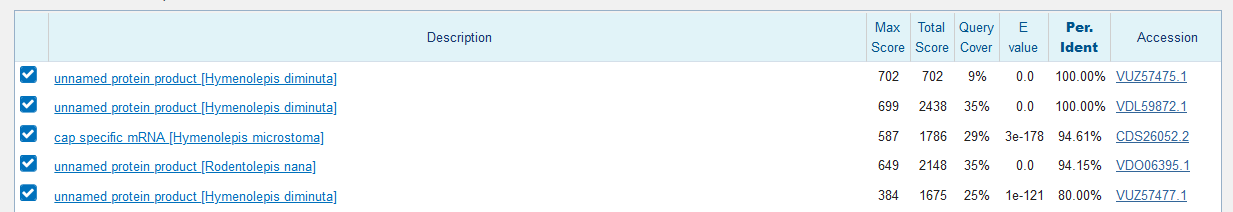
\includegraphics[width=1.0\textwidth]{result.png}
    \label{fig:result}
    \caption[]{Wyniki algorytmu BLASTX z bazy NCBI}
\end{figure}

\end{document}
